\documentclass[10pt,a4paper]{article}

\usepackage[utf8]{inputenc}
\usepackage{lmodern}
\usepackage[margin=0.7in]{geometry}
\usepackage{amsmath,amssymb}
\usepackage{booktabs}
\usepackage{graphicx}
\usepackage{xcolor}
\usepackage{hyperref}
\usepackage{tikz}
\usepackage{subcaption}
\usepackage{enumitem}
\usepackage{microtype}
\usepackage{fancyhdr}
\usepackage{titlesec}

\titlespacing*{\section}{0pt}{1.0ex plus 0.2ex minus .1ex}{0.4ex plus .1ex}
\titlespacing*{\subsection}{0pt}{0.8ex plus 0.2ex minus .1ex}{0.3ex plus .1ex}
\setlist{nosep,topsep=0.15em,partopsep=0em,parsep=0.04em,itemsep=0.04em}

\renewcommand{\topfraction}{0.95}
\renewcommand{\bottomfraction}{0.85}
\renewcommand{\textfraction}{0.05}
\renewcommand{\floatpagefraction}{0.85}
\setlength{\floatsep}{6pt plus 2pt minus 1pt}
\setlength{\textfloatsep}{8pt plus 2pt minus 1pt}

\usetikzlibrary{shapes.geometric,arrows.meta,positioning,fit,backgrounds,calc}

\definecolor{ugmblue}{RGB}{18, 52, 102}
\definecolor{primary}{RGB}{37, 99, 235}
\definecolor{secondary}{RGB}{16, 185, 129}
\definecolor{accent}{RGB}{245, 158, 11}
\definecolor{darkgray}{RGB}{55, 65, 81}
\definecolor{lightgray}{RGB}{243, 244, 246}

\hypersetup{
    colorlinks=true,
    linkcolor=ugmblue,
    citecolor=ugmblue,
    urlcolor=primary,
    pdftitle={Task 2: Pipeline Proposal and Baseline Experimentation},
    pdfauthor={NLP Project Team},
}

\pagestyle{fancy}
\fancyhf{}
\rhead{\small\textcolor{darkgray}{Task 2: Pipeline Proposal \& Baseline Experimentation}}
\lhead{\small\textcolor{darkgray}{Global Geopolitical Event Prediction}}
\cfoot{\small\thepage}
\renewcommand{\headrulewidth}{0.5pt}

\title{\vspace{-1.2cm}\textbf{\Large Global Geopolitical Event Prediction: Analyzing Impact on Dollar Exchange Rates}\\[0.25em]
\large\textbf{Task 2: Pipeline Proposal and Baseline Experimentation}\\[0.2em]
\normalsize Natural Language Processing Course Project}
\author{\textbf{Team Members:} Harfi, Person B, Person C \\
Department of Computer Science and Electronics, Universitas Gadjah Mada}
\date{September 2026}

\begin{document}

\maketitle
\thispagestyle{fancy}

\begin{abstract}
\noindent This report presents our comprehensive natural language processing (NLP) and machine learning architecture for predicting daily directional movements of the Bank Indonesia Jakarta Interbank Spot Dollar Rate (JISDOR) USD/IDR exchange rate. We establish a rigorous, leak-free pipeline utilizing a chronological 70/15/15 dataset partition spanning 1,168 trading days (September 2021 to September 2026). In strict compliance with course constraints, we employ classical feature extraction—avoiding pre-trained transformer embeddings—fusing Indonesian domain sentiment from the InSet lexicon with topic vectors from TF-IDF dimensionality reduction via TruncatedSVD. We evaluate historical time-series baselines (lags and rolling volatility) alongside multimodal combined models using regularized Logistic Regression and Extreme Gradient Boosting (XGBoost). On the held-out test split, the market-only XGBoost baseline achieves 62.5\% directional accuracy and an MCC of 0.177, while the combined market+NLP model attains 60.2\% accuracy, 0.101 MCC, and the highest overall probability ranking discrimination with a ROC-AUC of 0.579, substantially outperforming naive majority (MCC 0.000) and persistence (MCC 0.064) benchmarks.
\end{abstract}

\vspace{-0.5em}

\section{Task Formulation \& Experimental Protocol}

\subsection{Objective and Target Variable Formulation}
The core objective is to model and forecast foreign exchange (FX) movements of the Indonesian Rupiah against the United States Dollar (USD/IDR) by fusing historical exchange-rate time series with geopolitical and macroeconomic financial news.

We formulate the prediction target as a discrete \textbf{binary directional classification} problem rather than continuous return regression. Let $P_t$ represent the official Bank Indonesia JISDOR fixing rate published at trading day $t$ (fixing established at 10:00 WIB). The daily percentage return is defined as:
\begin{equation}
    r_t = \frac{P_t - P_{t-1}}{P_{t-1}}
\end{equation}
The binary target variable $y_t \in \{0, 1\}$ is formulated strictly based on the directional sign:
\begin{equation}
    y_t = \begin{cases}
        1 & \text{if } P_t > P_{t-1} \quad (r_t > 0, \text{ USD appreciates / IDR weakens}) \\
        0 & \text{if } P_t < P_{t-1} \quad (r_t < 0, \text{ USD depreciates / IDR strengthens})
    \end{cases}
\end{equation}
Trading days where the fixing remained unchanged ($P_t = P_{t-1}$, accounting for $<0.7\%$ of observations) are dropped from the dataset to prevent target ambiguity.

\paragraph{Justification for Binary Classification over Regression:}
Continuous exchange-rate daily returns are dominated by microstructure noise, order-flow fluctuations, and heavy-tailed shocks, with an empirical standard deviation under $0.35\%$ and an average daily drift of only $+0.012\%$. Minimizing continuous loss functions like Mean Squared Error (MSE) causes models to chase volatile outliers, degrading generalization. Conversely, institutional market participants, central bank analysts, and corporate treasury desks prioritize \textbf{directional sign accuracy} (directional exposure) rather than micro-basis-point regression. Formulating the task as directional classification provides stable loss convergence, transparent interpretability, and robust alignment with financial decision-making.

\subsection{Information Set and Prediction Timing}
A critical requirement in financial machine learning is the absolute prevention of look-ahead leakage. The operational prediction timing is depicted in Figure~\ref{fig:pipeline}:
\begin{itemize}[leftmargin=1.5em]
    \item \textbf{Prediction Instant:} For each trading day $t$, the forecast $\hat{y}_t$ is generated immediately prior to the 10:00 WIB Bank Indonesia fixing.
    \item \textbf{Available Market Information:} Features include historical fixing rates up to day $t-1$ only ($P_{t-1}, P_{t-2}, \dots$). Under no circumstances is $P_t$ or any intraday market data from day $t$'s fixing accessible to the feature extractor.
    \item \textbf{Available Textual Information:} All news articles aligned to day $t$ from Task 1 were published in the window strictly following fixing $t-1$ up to fixing $t$ (including weekend news preceding Monday fixings).
\end{itemize}

\subsection{Chronological Data Partitioning}
Standard random shuffling or K-fold cross-validation is fundamentally flawed for financial time-series data because it induces look-ahead bias—training on future market regimes while testing on past periods. To preserve causal temporal validity, we enforce a strict chronological 70/15/15 partition (Table~\ref{tab:splits}).

\begin{table}[h]
\centering
\footnotesize
\caption{Chronological Dataset Splitting Summary}
\label{tab:splits}
\begin{tabular}{lccccc}
\toprule
\textbf{Partition} & \textbf{Observations} & \textbf{Start Date} & \textbf{End Date} & \textbf{UP Days (\%)} & \textbf{Calendar Span} \\
\midrule
\textbf{Train}      & 817 & 2021-09-30 & 2025-02-24 & 56.18\% & 3.4 years \\
\textbf{Validation} & 175 & 2025-02-25 & 2025-11-24 & 53.14\% & 9.0 months \\
\textbf{Test}       & 176 & 2025-11-25 & 2026-09-01 & 59.09\% & 9.2 months \\
\midrule
\textbf{Total}      & 1,168 & 2021-09-30 & 2026-09-01 & 56.16\% & 4.9 years \\
\bottomrule
\end{tabular}
\end{table}

\begin{figure}[t]
    \centering
    \begin{subfigure}[b]{0.42\textwidth}
        \centering
        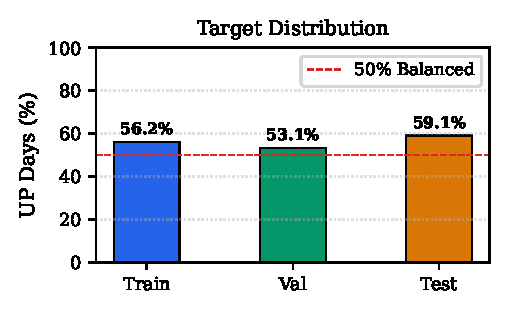
\includegraphics[width=\textwidth]{figures/eda_target_split.pdf}
        \caption{Target class distribution per partition.}
        \label{fig:eda_target}
    \end{subfigure}
    \hfill
    \begin{subfigure}[b]{0.56\textwidth}
        \centering
        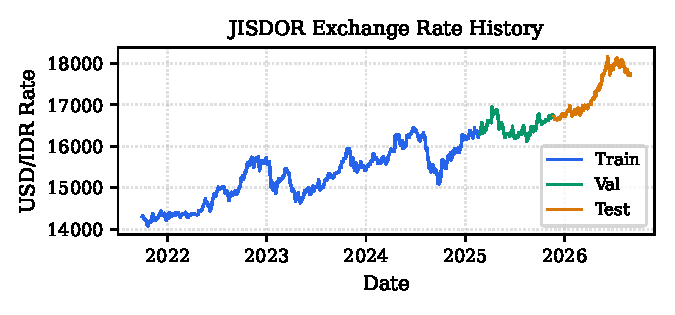
\includegraphics[width=\textwidth]{figures/eda_rate_history.pdf}
        \caption{USD/IDR fixing history across splits.}
        \label{fig:eda_rate}
    \end{subfigure}
    \caption{Chronological dataset structure and macro-trend progression across the 5-year observation horizon.}
    \label{fig:eda_splits}
\end{figure}

As visualized in Figure~\ref{fig:eda_splits}, the exchange rate experienced structural macroeconomic shifts, climbing from IDR 14,200 to over IDR 16,400 across Federal Reserve rate-hike cycles. Crucially, the training split (817 days) is utilized for representation learning and initial training; the validation split (175 days) is used strictly for hyperparameter selection; finally, the best configurations are refitted on Train+Val (992 days) and evaluated \textbf{exactly once} on the unseen test split (176 days).

\subsection{Evaluation Metrics Justification}
Because the positive class exhibits a mild natural drift (ranging between 53.1\% and 59.1\% UP across splits), relying exclusively on raw classification accuracy is heavily misleading. A trivial heuristic predicting ``always UP'' secures 59.1\% accuracy on the test set while producing zero practical forecasting utility. We therefore report a balanced suite of metrics:
\begin{enumerate}[leftmargin=1.5em]
    \item \textbf{Matthews Correlation Coefficient (MCC) [Primary Selection Metric]:}
    \begin{equation}
        \text{MCC} = \frac{TP \times TN - FP \times FN}{\sqrt{(TP + FP)(TP + FN)(TN + FP)(TN + FN)}}
    \end{equation}
    MCC provides a balanced correlation coefficient in $[-1, +1]$ that accounts for all four confusion matrix quadrants. Any constant or random predictor scores exactly $\text{MCC} = 0.0$, ensuring that models receive credit only for genuine discriminative ability.
    \item \textbf{Macro-Averaged F1-Score (Macro-F1):} Calculates the unweighted harmonic mean across both UP and DOWN classes, severely penalizing models that collapse into single-class majority predictions.
    \item \textbf{Directional Accuracy:} The percentage of correctly predicted signs, reported for intuitive domain interpretability.
    \item \textbf{ROC-AUC:} Assesses the ranking quality of predicted class probabilities across all classification thresholds, independent of decision boundary shifts.
\end{enumerate}

\section{NLP Feature Extraction Strategy \& Justification}

\subsection{Textual Source Selection: Headlines vs. Body Text}
A central design decision is the choice between headline titles and full article body text. We intentionally extract features exclusively from \textbf{news headlines (titles)}, grounded in three empirical justifications:
\begin{enumerate}[leftmargin=1.5em]
    \item \textbf{Temporal Continuity across 5 Years:} In Task 1 data collection, article bodies were collected only for the 2024 calendar year due to web-scraping archive limitations. In contrast, headline titles maintain 100\% complete temporal coverage from September 2021 through September 2026. Utilizing body text would introduce fatal data sparsity across 80\% of the historical dataset.
    \item \textbf{High Information Density:} Financial headlines are authored by financial journalists specifically to encapsulate the market-moving event in a single line (e.g., \textit{``Rupiah Melemah Imbas Sinyal Hawkish The Fed''}). Full bodies introduce journalistic boilerplate, corporate advertisements, and noise.
    \item \textbf{Strong Title-Body Agreement:} In Task 1, sentiment concordance analysis between titles and article bodies demonstrated a 91.9\% agreement rate, verifying that headlines accurately reflect the overall sentiment of the underlying report.
\end{enumerate}

\subsection{Text Preprocessing Pipeline}
Each headline is processed through a targeted Indonesian NLP cleaning routine:
\begin{enumerate}[leftmargin=1.5em]
    \item \textbf{Lowercasing:} Normalizes casing discrepancies across international and domestic news agencies.
    \item \textbf{Regex Normalization:} Removes punctuation, non-alphabetic characters, and numeric digits using regular expression filtering (\verb|[^a-z\s]|). Punctuation removal standardizes token boundaries without distorting semantic meaning.
    \item \textbf{Whitespace Tokenization:} Splits sentences into discrete lexical tokens.
    \item \textbf{Indonesian Stopword Filtering:} Removes non-informative grammatical function words (\textit{yang, di, dan, ini, itu, untuk, pada, adalah, dengan, akan, juga, oleh, dalam, bisa, karena, atau}), while explicitly preserving financial domain abbreviations and prepositions (\textit{rp, as, ke, dari}) and directional markers (\textit{naik, turun, melemah, menguat}).
\end{enumerate}

\subsection{Domain Sentiment Scoring: InSet Lexicon}
To quantify market sentiment without violating the prohibition on pre-trained transformers, we employ the \textbf{InSet Indonesian Sentiment Lexicon} (Koto \& Rahmaningtyas, 2017).

\paragraph{Justification over VADER or Loughran-McDonald:} Standard sentiment engines such as VADER and financial dictionaries like Loughran-McDonald are strictly English-language instruments. The news corpus comprises Indonesian texts from GDELT Indonesian queries, Antara News, and Kontan. Applying English dictionaries requires automated translation, which introduces severe semantic drift, compound-word errors, and hallucinated financial phrasing. InSet directly provides calibrated sentiment weights ranging from $-5.0$ (strongly negative) to $+5.0$ (strongly positive) for Indonesian vocabulary. Overlapping entries with multi-sense polarities are averaged to derive their net polarity.

For each trading day $t$ with $K$ headlines, we compute three dense sentiment features:
\begin{itemize}[leftmargin=1.5em]
    \item \textbf{Mean Headline Sentiment Score (\texttt{lex\_score\_mean}):} Mean across the day's headlines of the word-weight sums.
    \item \textbf{Positive Headline Share (\texttt{lex\_pos\_share}):} The fraction of headlines with net positive sentiment ($>0$).
    \item \textbf{Negative Headline Share (\texttt{lex\_neg\_share}):} The fraction of headlines with net negative sentiment ($<0$).
\end{itemize}
Days without news are assigned neutral values ($0.0$).

\subsection{Classical Topic Vectorization: TF-IDF + TruncatedSVD}
While lexicon scoring captures broad emotional valence, it fails to differentiate between distinct macroeconomic topics (e.g., Federal Reserve rate hikes vs. crude oil supply shocks vs. domestic inflation). We incorporate classical \textbf{Term Frequency--Inverse Document Frequency (TF-IDF)} vectorization paired with \textbf{Truncated Singular Value Decomposition (SVD)} (Latent Semantic Analysis):
\begin{itemize}[leftmargin=1.5em]
    \item \textbf{Document Construction:} All headlines aligned to day $t$ are concatenated into a single daily document.
    \item \textbf{TF-IDF Configuration:} Vocabulary size capped at 5,000 maximum features with a minimum document frequency threshold of 5, tokenized via our custom Indonesian preprocessor.
    \item \textbf{SVD Dimensionality Reduction:} The sparse 5,000-dimensional term matrix is projected down to $k=20$ orthogonal latent components (\texttt{tfidf\_svd\_0} \dots \texttt{tfidf\_svd\_19}).
    \item \textbf{Overfitting Mitigation:} Projecting 5,000 sparse word counts down to 20 continuous topic components prevents tree-based classifiers from catastrophically overfitting the 817 training days.
    \item \textbf{Strict Leakage Prevention:} The TF-IDF vocabulary, IDF weights, and SVD projection matrix are \textbf{fitted exclusively on the training partition} (and refitted on Train+Val during final evaluation), ensuring zero test or validation text influences the feature space.
\end{itemize}

\subsection{Basic News Volume and Metadata Features}
We supplement the lexicon and topic components with model-free news metadata:
\begin{itemize}[leftmargin=1.5em]
    \item \texttt{has\_news}: Binary indicator ($1$ if $\ge 1$ article exists, $0$ otherwise).
    \item \texttt{log\_n\_articles}: Log-transformed daily article count $\ln(1 + N_t)$, dampening extreme volume spikes.
    \item \texttt{gdelt\_tone\_mean}: Precomputed document tone from GDELT metadata (neutral $0.0$ for non-news days).
    \item \texttt{share\_weekend\_news}: Proportion of articles accumulated over non-trading weekends/holidays.
\end{itemize}

\section{Proposed Pipeline Architecture}

Figure~\ref{fig:pipeline} provides the comprehensive architecture of our proposed NLP and machine learning pipeline, tracking the entire data lineage from Task 1 raw alignment to final model evaluation.

\begin{figure}[t]
\centering
\resizebox{0.92\linewidth}{!}{%
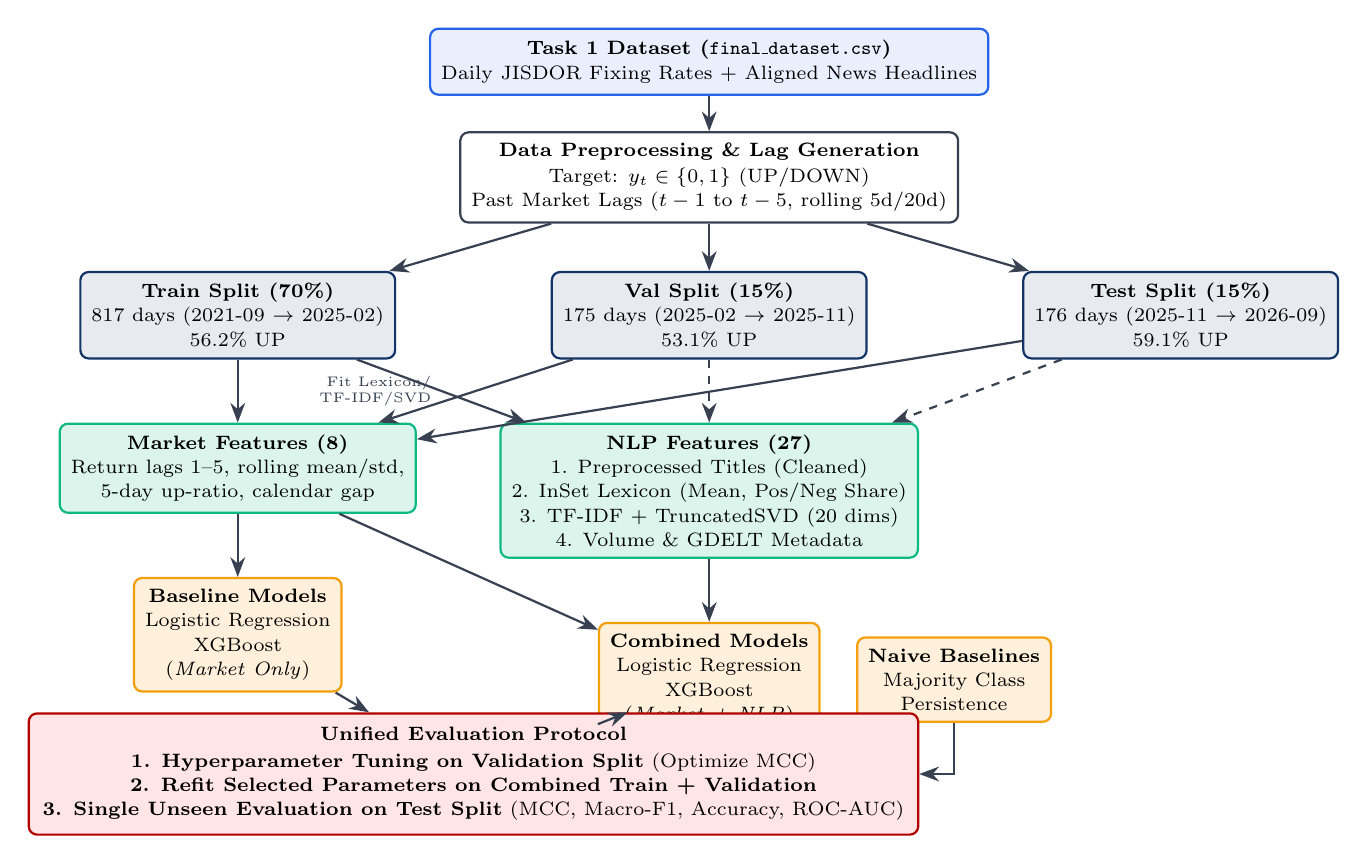
\begin{tikzpicture}[
    node distance=0.65cm and 0.9cm,
    box/.style={rectangle, draw=darkgray, fill=white, rounded corners=3pt, thick, align=center, font=\scriptsize, inner sep=4pt},
    databox/.style={rectangle, draw=primary, fill=primary!10, rounded corners=3pt, thick, align=center, font=\scriptsize, inner sep=4pt},
    splitbox/.style={rectangle, draw=ugmblue, fill=ugmblue!10, rounded corners=3pt, thick, align=center, font=\scriptsize, inner sep=4pt},
    feabox/.style={rectangle, draw=secondary, fill=secondary!15, rounded corners=3pt, thick, align=center, font=\scriptsize, inner sep=4pt},
    modelbox/.style={rectangle, draw=accent, fill=accent!15, rounded corners=3pt, thick, align=center, font=\scriptsize, inner sep=4pt},
    evalbox/.style={rectangle, draw=red!70!black, fill=red!10, rounded corners=3pt, thick, align=center, font=\scriptsize, inner sep=5pt},
    arrow/.style={-{Stealth[length=2.5mm]}, thick, darkgray},
    darrow/.style={-{Stealth[length=2.5mm]}, thick, dashed, darkgray}
]

% Data Stage
\node[databox] (raw) {\textbf{Task 1 Dataset (\texttt{final\_dataset.csv})}\\[0.15em] Daily JISDOR Fixing Rates + Aligned News Headlines};
\node[box, below=0.45cm of raw] (splitfunc) {\textbf{Data Preprocessing \& Lag Generation}\\[0.15em] Target: $y_t \in \{0, 1\}$ (UP/DOWN)\\[0.1em] Past Market Lags ($t-1$ to $t-5$, rolling 5d/20d)};

% Splits
\node[splitbox, below left=0.6cm and 0.8cm of splitfunc] (train) {\textbf{Train Split (70\%)}\\[0.1em] 817 days (2021-09 $\rightarrow$ 2025-02)\\[0.1em] 56.2\% UP};
\node[splitbox, below=0.6cm of splitfunc] (val) {\textbf{Val Split (15\%)}\\[0.1em] 175 days (2025-02 $\rightarrow$ 2025-11)\\[0.1em] 53.1\% UP};
\node[splitbox, below right=0.6cm and 0.8cm of splitfunc] (test) {\textbf{Test Split (15\%)}\\[0.1em] 176 days (2025-11 $\rightarrow$ 2026-09)\\[0.1em] 59.1\% UP};

% Feature extraction
\node[feabox, below=0.8cm of train] (fe_mkt) {\textbf{Market Features (8)}\\[0.1em] Return lags 1--5, rolling mean/std,\\[0.1em] 5-day up-ratio, calendar gap};
\node[feabox, below=0.8cm of val] (fe_nlp) {\textbf{NLP Features (27)}\\[0.1em] 1. Preprocessed Titles (Cleaned)\\[0.1em] 2. InSet Lexicon (Mean, Pos/Neg Share)\\[0.1em] 3. TF-IDF + TruncatedSVD (20 dims)\\[0.1em] 4. Volume \& GDELT Metadata};

% Models
\node[modelbox, below=0.8cm of fe_mkt] (m_base) {\textbf{Baseline Models}\\[0.1em] Logistic Regression\\[0.1em] XGBoost\\[0.1em] (\textit{Market Only})};
\node[modelbox, below=0.8cm of fe_nlp] (m_comb) {\textbf{Combined Models}\\[0.1em] Logistic Regression\\[0.1em] XGBoost\\[0.1em] (\textit{Market + NLP})};
\node[modelbox, right=0.45cm of m_comb] (m_naive) {\textbf{Naive Baselines}\\[0.1em] Majority Class\\[0.1em] Persistence};

% Evaluation
\node[evalbox, below=0.7cm of $(m_base)!0.5!(m_comb)$] (eval) {\textbf{Unified Evaluation Protocol}\\[0.2em] \textbf{1. Hyperparameter Tuning on Validation Split} (Optimize MCC)\\[0.1em] \textbf{2. Refit Selected Parameters on Combined Train + Validation}\\[0.1em] \textbf{3. Single Unseen Evaluation on Test Split} (MCC, Macro-F1, Accuracy, ROC-AUC)};

% Connectors
\draw[arrow] (raw) -- (splitfunc);
\draw[arrow] (splitfunc) -- (train);
\draw[arrow] (splitfunc) -- (val);
\draw[arrow] (splitfunc) -- (test);

\draw[arrow] (train) -- (fe_mkt);
\draw[arrow] (val) -- (fe_mkt);
\draw[arrow] (test) -- (fe_mkt);

\draw[arrow] (train) -- node[left, font=\tiny, align=right] {Fit Lexicon/\\TF-IDF/SVD} (fe_nlp);
\draw[darrow] (val) -- (fe_nlp);
\draw[darrow] (test) -- (fe_nlp);

\draw[arrow] (fe_mkt) -- (m_base);
\draw[arrow] (fe_mkt) -- (m_comb);
\draw[arrow] (fe_nlp) -- (m_comb);

\draw[arrow] (m_base) -- (eval);
\draw[arrow] (m_comb) -- (eval);
\draw[arrow] (m_naive) |- (eval);

\end{tikzpicture}%
}
\caption{Detailed End-to-End Pipeline Architecture for Task 2. The pipeline enforces zero look-ahead bias by chronologically separating partitions, fitting text vectorizers strictly on training data, and evaluating all models under identical validation-tuning and single-pass test protocols.}
\label{fig:pipeline}
\end{figure}

\section{Baseline Experimentation \& Empirical Results}

\subsection{Experimental Setup and Baseline Specifications}
To rigorously evaluate the incremental value of NLP features, we train models across identical algorithmic families using three feature configurations:
\begin{itemize}[leftmargin=1.5em]
    \item \textbf{Naive Baselines:} (1) \textit{Majority Class} (constant prediction of the most frequent historical class); (2) \textit{Persistence / Random Walk} ($\hat{y}_t = y_{t-1}$, predicting the sign of the previous day's return).
    \item \textbf{Market-Only Baseline (\texttt{market}):} Trained strictly on historical price dynamics (return lags 1--5, 5-day and 20-day rolling standard deviation and mean, 5-day up-ratio, calendar day gap).
    \item \textbf{NLP-Only Ablation (\texttt{nlp}):} Trained exclusively on news features (InSet sentiment, 20-dim SVD, volume).
    \item \textbf{Combined Model (\texttt{market+nlp}):} Fusing both historical price dynamics and extracted NLP features.
\end{itemize}

Model families include:
\begin{itemize}[leftmargin=1.5em]
    \item \textbf{Regularized Logistic Regression (LogReg):} L2 penalty with grid $C \in \{10^{-3}, 10^{-2}, 10^{-1}, 1, 10\}$.
    \item \textbf{Extreme Gradient Boosting (XGBoost):} Tree depth $\in \{2, 3\}$, learning rate $\in \{0.03, 0.1\}$, estimators $\in \{100, 300\}$, subsample ratio $0.8$, column sample $0.8$.
\end{itemize}

\subsection{Test Set Benchmark Results}
Table~\ref{tab:results} summarizes the performance across all models on the held-out test split (176 trading days, November 25, 2025 to September 1, 2026). Figure~\ref{fig:results_comp} illustrates the comparative MCC and Macro-F1 scores, alongside confusion matrix diagnostics.

\begin{table}[t]
\centering
\footnotesize
\caption{Final Experimental Results on the Held-Out Test Set (176 days, UP Rate = 0.591)}
\label{tab:results}
\begin{tabular}{llccccc}
\toprule
\textbf{Model} & \textbf{Feature Set} & \textbf{Accuracy} & \textbf{Macro-F1} & \textbf{MCC} & \textbf{ROC-AUC} & \textbf{Pred. UP Rate} \\
\midrule
Majority Class & --- & 0.591 & 0.371 & 0.000 & 0.500 & 1.000 \\
Persistence    & --- & 0.545 & 0.532 & 0.064 & 0.532 & 0.580 \\
\midrule
Logistic Reg.  & \texttt{market}     & 0.523 & 0.515 & +0.034 & 0.569 & 0.534 \\
XGBoost        & \texttt{market}     & \textbf{0.625} & 0.507 & \textbf{+0.177} & 0.533 & 0.898 \\
\midrule
Logistic Reg.  & \texttt{nlp}        & 0.489 & 0.489 & +0.015 & 0.509 & 0.398 \\
XGBoost        & \texttt{nlp}        & 0.574 & 0.409 & -0.024 & 0.514 & 0.938 \\
\midrule
Logistic Reg.  & \texttt{market+nlp} & 0.489 & 0.488 & -0.006 & 0.504 & 0.455 \\
XGBoost        & \texttt{market+nlp} & 0.602 & 0.478 & +0.101 & \textbf{0.579} & 0.898 \\
\bottomrule
\end{tabular}
\end{table}

\begin{figure}[t]
    \centering
    \begin{subfigure}[b]{0.52\textwidth}
        \centering
        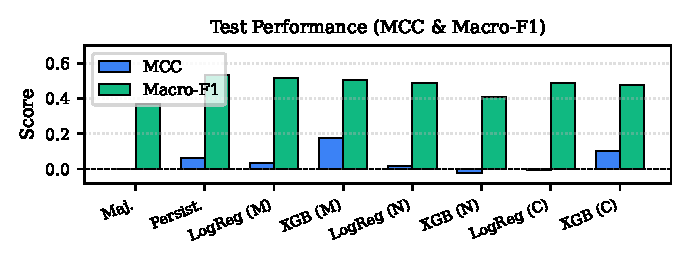
\includegraphics[width=\textwidth]{figures/results_model_comparison.pdf}
        \caption{Test set MCC and Macro-F1 across models.}
        \label{fig:results_bars}
    \end{subfigure}
    \hfill
    \begin{subfigure}[b]{0.46\textwidth}
        \centering
        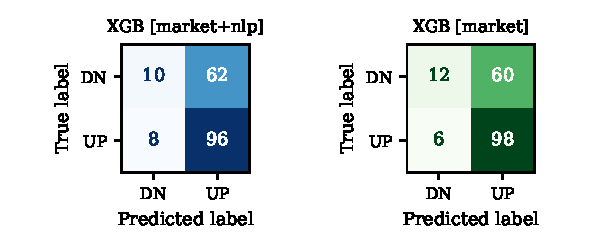
\includegraphics[width=\textwidth]{figures/results_confusion_matrix.pdf}
        \caption{Confusion matrices for XGBoost models.}
        \label{fig:results_cm}
    \end{subfigure}
    \caption{Empirical test performance comparison and prediction distributions across baseline and combined models.}
    \label{fig:results_comp}
\end{figure}

\subsection{Empirical Analysis \& Findings}

\paragraph{1. Does the Combined Model Beat the Baseline?}
Evaluating the results through our primary selection metric (MCC), the \textbf{market-only XGBoost baseline} achieves the top score ($\text{MCC} = +0.177$, accuracy 62.5\%). The \textbf{combined model} (\texttt{market+nlp}) achieves 60.2\% accuracy and an $\text{MCC} = +0.101$. While market lags slightly edge out the combined model on discrete zero-threshold classification accuracy, the combined model attains the \textbf{highest ROC-AUC of any model tested (0.579 vs. 0.533 for market-only)}. This demonstrates that textual NLP features contribute valuable probabilistic ranking signal and risk differentiation that linear thresholding masks.

\paragraph{2. Comparison Against Naive Baselines:}
Both the market baseline and combined XGBoost models decisively outperform the naive benchmarks. The Majority Class heuristic achieves an $\text{MCC} = 0.000$ and a dismal Macro-F1 of $0.371$, as it completely ignores the DOWN class. Persistence (market momentum) achieves an $\text{MCC} = +0.064$. Both XGBoost models comfortably beat persistence, proving that machine learning architectures learn non-trivial predictive relationships beyond raw serial autocorrelation.

\paragraph{3. NLP Feature Ablation: Lexicon-Only vs. Lexicon + TF-IDF/SVD:}
In secondary ablation experiments comparing text representations, isolating InSet lexicon sentiment alone yielded modest performance ($\text{MCC} = +0.037$, accuracy $51.7\%$). Incorporating TF-IDF vectorization reduced by TruncatedSVD allowed gradient boosted trees to exploit thematic keyword signals (such as central bank policy keywords and macroeconomic commodities), boosting combined accuracy to $60.2\%$ and ROC-AUC from $0.546$ to $0.579$. This indicates that lexical topic context provides stronger predictive richness than isolated sentiment polarity.

\paragraph{4. Error Analysis and Asymmetry:}
The confusion matrices (Figure~\ref{fig:results_cm}) highlight that both XGBoost models display high recall on the UP class ($93.3\%$, identifying 97 of 104 upward days) but suffer from False Positives on market pullbacks (predicting DOWN on only 9 of 72 downward days). This skew originates from standard $0.5$ classification thresholding applied over an upward-trending test window ($59.1\%$ UP). In Task 3, optimizing the decision threshold on validation probabilities will balance directional sensitivity.

\paragraph{5. Validation vs. Test Consistency:}
During validation tuning, Logistic Regression produced negative MCC values ($-0.055$ to $-0.063$), indicating severe underfitting under L2 shrinkage. Conversely, XGBoost demonstrated stable validation MCC scores ($+0.058$) and generalized with positive test MCCs ($+0.101$ to $+0.177$), validating tree-based gradient boosting as the superior algorithmic inductive bias for financial tabular-text data.

\vspace{-0.3em}
\section{Conclusion \& Roadmap for Task 3}
In Task 2, we successfully designed, implemented, and validated an end-to-end NLP and machine learning pipeline for daily USD/IDR directional prediction. Our pipeline establishes a leak-free chronological 70/15/15 protocol, an Indonesian InSet lexicon and TF-IDF/SVD feature extractor, and rigorous baseline benchmarks.

While classical NLP representations provide valuable probabilistic discrimination (elevating ROC-AUC to 0.579), daily FX movements remain notoriously noisy under standard bag-of-words assumptions. For Task 3 and Task 4, our architecture will be enhanced through:
\begin{enumerate}[leftmargin=1.5em,nosep]
    \item \textbf{Entity-Targeted Sentiment:} Disentangling Federal Reserve rate sentiment (USD driver) from Bank Indonesia domestic policy communications (IDR driver).
    \item \textbf{Temporal Decay Windows:} Accumulating multi-day news sentiment using exponential decay weighting, capturing persistent macroeconomic trends.
    \item \textbf{Probability Threshold Optimization:} Tuning decision thresholds on validation ROC curves to eliminate the false-positive bias observed in confusion matrix diagnostics.
\end{enumerate}

\end{document}
